\documentclass[a4paper,14pt,russian]{extreport}
 
\usepackage{extsizes}
\usepackage{cmap} % для кодировки шрифтов в pdf
\usepackage[T2A]{fontenc}
%\usepackage{pscyr}
%\renewcommand{\rmdefault}{ftm} % Times New Roman
\usepackage[utf8]{inputenc}
\usepackage[russian]{babel}
\usepackage{longtable}

\usepackage[pdfborder={0 0 0}]{hyperref}
  
\usepackage{graphicx} % для вставки картинок
\usepackage{amssymb,amsfonts,amsmath,amsthm} % математические дополнения от АМС
\usepackage{indentfirst} % отделять первую строку раздела абзацным отступом тоже
\usepackage[usenames,dvipsnames]{color} % названия цветов
\usepackage{makecell}
\usepackage{multirow} % улучшенное форматирование таблиц
\usepackage{ulem} % подчеркивания

\usepackage[left=2.5cm,right=2cm, top=2cm,bottom=2cm]{geometry} %Установка полей
\parindent=1.27cm
 
\linespread{1.3} % полуторный интервал
\frenchspacing

%\newtheorem{Def}{Определение} %Окружение для определения

\renewcommand{\labelenumi}{\arabic{enumi}.}
\renewcommand{\labelenumii}{\arabic{enumi}.\arabic{enumii}.}
\renewcommand{\labelenumiii}{\arabic{enumi}.\arabic{enumii}.\arabic{enumiii}.}
\renewcommand{\figurename}{Рисунок}
\renewcommand{\thefigure}{\arabic{figure}}

%Глава
\makeatletter
\renewcommand{\@makechapterhead}[1]{
%\vspace*{0 pt}
	{\normalfont
	\thechapter\quad
	\normalfont #1\par
	
	%\nopagebreak
	\vspace{3ex}}
}

\renewcommand{\@makeschapterhead}[1]{
%\vspace*{0 pt}
	{\normalfont
	\normalfont #1\par
	
	%\nopagebreak
	\vspace{3ex}}
}

%Переопределение нумераций и стилей рубрикаций
\renewcommand{\thesection}{\arabic{chapter}.\arabic{section}}
\renewcommand{\section}{\@startsection{section}{1}{\parindent}{3ex}{3ex}{\normalfont}}

\renewcommand{\thesubsection}{\arabic{chapter}.\arabic{section}.\arabic{subsection}}
\renewcommand{\subsection}{\@startsection{subsection}{2}{\parindent}{3ex}{3ex}{\normalfont}}

\renewcommand{\thesubsubsection}{\arabic{chapter}.\arabic{section}.\arabic{subsection}.\arabic{subsubsection}}
\renewcommand{\subsubsection}{\@startsection{subsubsection}{3}{\parindent}{3ex}{3ex}{\normalfont}}

%Переопределение стилей списков
\renewcommand{\@listI}{\topsep=0cm\parsep=0cm\partopsep=0cm\itemsep=0cm\leftmargin=0cm\itemindent=1.27cm}

%Стили оглавления
\renewcommand{\l@chapter}{\@dottedtocline{0}{0em}{3em}}
\renewcommand{\l@section}{\@dottedtocline{1}{0em}{3em}}
\renewcommand{\l@subsection}{\@dottedtocline{2}{0em}{3em}}

%Переопределение подписи рисунка
\renewcommand{\@makecaption}[2]{\vspace{\abovecaptionskip}\sbox{\@tempboxa}{#1: #2}%
\ifdim \wd\@tempboxa >\hsize
	#1. #2\par
\else
	\global\@minipagefalse
	\hbox to \hsize {\hfil #1. #2\hfil}%
\fi
\vspace{\belowcaptionskip}}

\renewcommand{\@biblabel}[1]{#1.\hfill}

%Переопределение надписи таблицы
\makeatother
 
\begin{document}
Первый
\newpage
Второй
\newpage
\chapter*{Аннотация}

ТОНАЛЬНОСТЬ ДОКУМЕНТА, НЕЧЕТКАЯ ЛОГИКА, ИНФОРМАЦИОННОЕ ПОЛЕ

В данной работе рассматривается задача оценки тональности некоторого набора документов и предпринимается попытка обосновать разработанные алгоритмы оценки тональности общего информационного поля.

Для решения проблемы поэтапно рассматриваются следующие задачи: обзор и анализ существующих методов и алгоритмов оценки тональности документа и, соответственно, информационного поля; реализация составления словаря тональностей отдельных лексических единиц, рассмотрение алгоритма общей оценки информационного поля по некоторому количеству документов.

Для проверки обоснованности определенных методов разрабатывается программная реализация решения данной задачи, проводится применение определенных методов и исследование полученных результатов.

В качестве требуемых для решения данной задачи дисциплин определены следующие: нечеткая логика, линейная алгебра, математическая статистика, объектно-ориентированное программирование, алгоритмические языки, системы управления базами данных, операционные системы и среды.

\begin{center}
ГРАФИЧЕСКАЯ ЧАСТЬ
\end{center}

Плакат 1. Постановка задачи

Плакат 2. Синтаксический анализ предложения

Плекат 3. Представление предложения как набора синтаксических единиц

Плакат 4-8. Определение эмоциональной тональности синтаксической единицы

Плакат 9. Аннотирование. Базовый алгоритм

Плакат 10. Аннотирование. Алгоритм LRU-K

Плакат 11. Оценка тональности документа

Плакат 12. Программа <<Оценка тональности информационного поля>>

Плакат 13.Результаты

\medskip\hrule\medskip

Всего плакатов\dotfill 13
\newpage
\tableofcontents
\newpage
\chapter*{Введение}
\addcontentsline{toc}{chapter}{Введение}
В настоящее время одну из ведущих ролей в качестве фактора развития общества занимает информационная среда, являющая собой совокупность информации, информационной инфраструктуры, а также субъектов, осуществляющих сбор, структуризацию и тиражирование информации. Активно влияя на политику, экономику, социум и многие другие факторы, информационная сфера является одним из системообразующих факторов жизни и функционирования общества.

Сегодня информационная сфера является системообразующим фактором жизни общества: она активно влияет на политическую, экономическую, социальную и другие составляющие.

Также в условиях глобализации экономики информационная борьба набирает все большие обороты. Она ведется явно и скрыто между государствами, предприятиями и фирмами в защиту собственных интересов, разделения зон влияния. Очевидно, что для того, чтобы эффективно противодействовать конкурентам, необходимо знать, против кого и против чего действовать в конкретных условиях, и какими средствами обеспечивать это противодействие.

Проблемы оценки конкурентной среды обращали на себя внимание многих поколений практиков. Для противодействия конкурентам, эффективного проведения рекламной и PR-деятельности создавались и применялись модели анализа и оценки конкурентной среды с различными допущениями. Однако и в настоящее время, в связи с развитием сети Интернет, этот вопрос остается открытым.

Мнения влияют на решения людей. В настоящее время каждый человек перед принятием решения о выборе поставщика, покупке какой-нибудь дорогостоящей вещи, выборе места отдыха или учебного заведения для своего ребенка и т.д. изучает отзывы и обзоры в сети Интернет.

В связи с этим возникает необходимость оперативно и качественно отслеживать информационное поле и выявлять субъективный образ объекта, естественно возникающий или намеренно формируемый в сети Интернет и СМИ.

Начиная с момента своего появления и до настоящего времени Интернет занимает позиции одного из основных информационных источников. Доля пользователей Интернета в мире составляет 35\%, причем в развитых странах доля вплотную приблизилась к 50\% населения.  В то же время, благодаря своей обособленности и относительной анонимности, Интернет является источником более объективной (в сумме) информации. Россия на данный момент занимает лидирующее место в Европе по количеству пользователей как в абсолютном, так и в процентном показателях. Пользователи пишут статьи и заметки, выражая свое мнение о приобретенных и полученных товарах и услугах, их производителях и других потребителях благ (что, в целом, тоже важно) на форумах, в социальных сетях и блогах.
%\begin{Def}
Определение. Образ, формируемый в СМИ и сети Интернет, называют информационным полем \mbox{(ИП)} объекта.
%\end{Def}

%\begin{Def}
Определение. Под тональностью информационного поля \mbox{(ТИП)} понимается обобщенная оценка тональности найденных текстов с целью выявления эмоциональной оценки авторов по отношению к объекту исследования.
%\end{Def}

Вовремя оценивая и проводя мониторинг \mbox{ТИП}, можно существенно повысить качество предоставляемых товаров и услуг, эффективно влияя на образ исследуемого предмета.

Задача данного типа может найти весомое применение в следующих областях:

\begin{itemize}
\item Мониторинг СМИ;
\item Социологические исследования;
\item Конкурентная разведка;
\item Информационные войны;
\item Оценка эффективности PR-компаний;
\item Рекомендательные системы.
\end{itemize}

Целью данной дипломной работы является разработка методики подокументной оценки \mbox{ТИП} некоторого объекта. Для достижения результата требуется решить несколько последовательных задач:

\begin{enumerate}
\item Обзор и анализ существующих методов и реализаций оценки \mbox{ТИП} некоторого документа;
\item Классификация существующих методов с подбором наиболее оптимальных;
\item Компоновка конечного математического аппарата с обоснованием выбора каждой составной части;
\item Решение задачи c помощью исследованных методов и разработанного \mbox{ПО}; анализ полученных результатов.
\end{enumerate}

Практический смысл работы выражается в применении полученного математического аппарата и \mbox{ПО} к анализу ТИП некоторого объекта.

Методика исследования

В работе применены методы таких областей, как линейная алгебра, нечеткая логика, математическая статистика, \mbox{ООП}, операционные системы и среды, \mbox{СУБД}.

Разработанное ПО позволяет производить автоматизированную оценку \mbox{ТИП} некоторого объекта.

В частности, данная модель была применена к оценке \mbox{ТИП} \mbox{ФГБОУ} \mbox{ВПО} <<Липецкий государственный технический университет>>, в результате чего была получена оценка \mbox{ТИП} на основе некоторого множества уникальных документов.

Данная работа разбита на введение, 4~главы и заключение, общий объем составляет 80~страниц.

В первой части рассмотрены этапы развития методик решения поставленной задачи, анализируется необходимый математический аппарат, дается попытка обоснования выбранного подмножества моделей и методов, разрабатывается общий алгоритм решения и дается его обоснование.

Во второй части рассматриваются уже сами математические модели, производится их классификация, приводится математический вид алгоритма решения.

В третьей части приведено описание созданного программного продукта. Рассмотрена структура программы, функционал и приложено руководство пользователя.

Четвертая часть посвящена анализу \mbox{ТИП} \mbox{ЛГТУ} с помощью разработанных моделей и \mbox{ПО}, применению по для проведения указанной оценки.

В заключении приведены выводы по работе, а также оценены перспективы как созданного программного продукта, так и математического аппарата.
\newpage

\chapter{Обзор методик решения задач оценки ТИП, документа, получения средневзвешенной оценки, разбор проблем}

При решении задач данного типа возникает необходимость четкого определения набора необходимых методов решения.

В качестве входных данных используется некоторый набор документов, в котором заведомо присутствуют упоминания оцениваемого объекта. Для каждого документа путем лексического разбора определяются атомарные составные части, для которых определена исходная тональность по некоторой шкале. Производится суммирование тональностей и вычисление оценки всего текста. И, наконец, проведя средневзвешенную оценку всех тональностей, получим общую \mbox{ТИП} объекта.

В общем, ставится задача оценки \mbox{ТИП} документа в конструктивной постановке как последовательность следующих операций с текстом:

\begin{enumerate}
\item Поиск всех упоминаний об объекте в тексте, включая его синонимы и аббревиатуры (данный этап может и не проводиться, если заведомо известно, что документы относятся к объекту);
\item Синтаксический разбор текста для определения атомарных частей, выявление связей между ними;
\item Выделение позиций с ярко выраженной тональностью.
\item Определение тональности для каждой позиции и суммирование тональностей для определения общей оценки.
\end{enumerate}

Ниже разберем подробнее историю развития и сами методы оценки \mbox{ТИП}.

\section{Обзор методов синтаксического анализа и разбора}
Определим набор функций, который должен поддерживать стандартный синтаксический анализатор:

\begin{enumerate}
\item разбор исходного текста с применением лексического и морфологического анализа;
\item определение контекстно-свободной составляющей текста;
\item построение синтаксического дерева;
\item уведомление об ошибках.
\end{enumerate}

Одним из основных вопросов в области компьютерной лингвистики принимается задача об очереди синтаксического этапа в определении структуры текста. Стоит отметить, что из двух наиболее общепринятых подходов к построению систем в данном случае следует принять модульный подход, так как он позволит обеспечить произвольную и независимую компоновку основных частей, в т.~ч. и синтаксического анализатора

Создавая компонент синтаксического анализатора, прежде всего возникает надобность в построении синтаксической модели естественного языка, для чего определяются следующие наборы правил:

\begin{itemize}
\item методики описания синтаксиса языка;
\item способы представления синтаксической структуры предложения;
\item методики анализа и синтеза приложений на естественном языке;
\end{itemize}

Переходя к выбору способа представления синтаксической модели, определим следующие модели построения синтаксической структуры.

\subsection{Дерево зависимостей}

Данная структура определена как наиболее часто используемая, в частности, благодаря тому, что опыт разработки языков программирования был перенесен на анализ естественных языков. Данный способ также является наиболее наглядным.

Некоторое предложение представлено как линейно упорядоченное множество элементов (словоформ), на основании которого строится ордерево (узлы~-- элементы множества). Дуги представляют собой подчинительную связь, чье направление совпадает с дуговым.

Древовидные структуры обладают одним немаловажным свойством, а именно проективностью, т.~е. способностью отразить связь между линейной структурой предложения и отношениями подчинения между его частями, что в результате позволяет определить зависимости и добиться более точного анализа в широком спектре прикладных задач. Данное свойство легко просматривается при графическом построении дерева зависимостей.

Дерево является полностью проективно зависимым, если для любых трех его узлов выполняется отношение транзитивности зависимостей. Для слабопроективных предложений две пары зависимостей $\left(a, b\right)$ и $\left(c, d\right)$ не разделяют друг друга. Следует отметить, что для делового и повсеместного повседневного стиля характерно использование в основном проективных предложений, т.~е. можно утверждать с большой долей вероятности $\left(\sim78,9\%\right)$, что большинство современных синтаксических анализаторов в состоянии построить адекватную синтаксическую модель (дерево зависимостей) для большей части источников всемирной паутины.

Модель не лишена недостатков:

\begin{enumerate}
\item использование лишь подчинительных связей;
\item каждое слово формально рассматривается как отдельный элемент предложения;
\end{enumerate}

Если первое ограничение в свете вышеуказанных причин не особенно влияет на конечный результат (так как в в корпусе русского языка используются в основном подчинительные связи), то второе ограничение явно не говорит в пользу предложенной модели, т.~к. в самих предложениях некоторые части м.~б. связаны сочинительно (имена собственные, обороты и т.~д.).

\subsection{НС-структуры}

НС-структура (структуры непосредственно составляющих)~-- некоторое множество отрезков предложения, которые удовлетворяют следующим условиям~\cite{volk}:

\begin{itemize}
\item за элементы множества принимают само предложение и его отдельные словоформы;
\item составляющие состоят из непосредственно связянных синтаксически отрезков;
\item составляющие не образуют пересечений или одна полностью входит в другую.
\end{itemize}

НС-структуры формируют синтаксически связанные части предложений (в т.~ч. и отдельные слова), определенные как единое целое (сочинительные отношения).

Модели присущи следующие недостатки:

\begin{itemize}
\item Связи между элементами неоднозначны;
\item Не применяются иерархии внутри частей одного уровня;
\item Нет возможности отображения непроективных предложений;
\end{itemize}
\subsection{ОНС-структуры}
В ОНС-структурах (ориентированные НС-структуры) одна из составляющих трактуется как главная для некоторой неодноэлементной составляющей~\cite{volk}.

Всякая такая структура определяет соответствующее ей дерево зависимостей или НС-структуру.

Неподчинительные связи описываются зачастую неверно.
\subsection{ЧОНС-структуры}
В отличие от ОНС-структур, в данной модели (частично ориентированные НС-стуктуры) не к каждому элементу применяется выделение главной части (только для некоторого подмножества)~\cite{volk}.

Это позволяет описывать как подчинительные, так и сочинительные связи, что позволяет отразить богатый набор связей и сочетаний (например, обороты, имена собственные, предложные связи).
\section{Методы оценки тональностей атомарных частей текста}

Для проведения анализа тональности текста (отдельных его предложений), требуется оценить тональности его атомарных частей (слов). Само собой, для этого не существует универсального математического метода.

В качестве единственно возможного подхода здесь предлагается разработать частично автоматизированную систему, реализующую составление ассоциативного словаря тональностей.

Данный этап представляет собой сбор подготовительных данных, и, по сути, выполняется до начала всех остальных.

В некоторых изданиях предлагается методика, согласно которой для определенной предметной области словарь составляется вручную, и каждому слову сопоставляется определенная тональная оценка: <<позитивно>> или <<негативно>>. Такой алгоритм не является универсальным.

Иначе проблема решаема при помощи разработки методов оценки тональности, полагаясь на ассоциативное восприятие изображений человеком.

На данном этапе развития веб-сервисов для облегчения навигации, категоризации и тематического поиска пользователи расставляют теги (метки), характеризующие содержимое изображения. Т.~о., это позволяет ассоциировать набор слов ЕЯ с изображением. У человека, просматривающего данное изображение, возникает некоторая его тональная оценка, распостраняемая и на теги изображения.

В качестве шкалы тональности зачастую используется бинарная система, <<позитивно>>-<<негативно>> (иногда добавляется <<нейтрально>>). Но такая градация является слишком резкой, не позволяя тональность в полной мере.

Выход состоит в том, чтобы использовать небинарную ранговую тональную шкалу (оперируя более широким числом градаций), и методы нечеткой логики как при оценке, так и при агрегации нескольких пользовательских оценок.

Некоторый акцент следует сделать на проблеме агрегации. При проведении оценок некоторого слова несколькими пользователями неизбежно ставится вопрос о извлечении некоторой общей оценки для слова. В данном случае предлагается использовать аппарат математической статистики.
\section{Обзор методов определения тональности текста}

После проведения синтаксического анализа предложений в тексте мы получаем данные о структуре предложения. Эти данные вкупе со словарем тональностей используются для определения тональности уже целого текста.

В ряде публикаций, в частности , приводятся алгоритмы определения тональности текста по уже сформированным словарям тональностей.

Во многих из них предполагается использование эмоциональных тональностей, определенных на уровне некоторых лексем. Агрегируя тональности отдельных лексем, применяя правила их сочетания, получаем общую лексическую тональность текста.

Также при проведении оценки тональности текста подразумевается выделение тех частей текста, которые выражают отношение к объекту по шкале тональности.

В частности, в работах определены следующие методы оценки тональности текстов~\cite{gubin}

\begin{enumerate}
\item Текст оценивается с помощью аппарата векторного анализа, применяя размеченный эталонный корпус. Полученный результат на основе сравнения относится к позитиву или к негативу.
\item Тональность определяется на основе методов лингвистического анализа с применением тональных словарей. В совокупности текст может быть оценен по шкале тональностей, отражающей количество лексики для градаций. В данной работе используется именно этот подход.
\item Комбинация методов.
\end{enumerate}

Первый метод при весьма высокой скорости работы требует наличия предварительно размеченного эталонного корпуса, на основе которого происходит обучение создание схем для алгоритма. Недостатками такого метода является огромная трудоемкость адекватно размеченного корпуса для русского языка. К этому следует добавить, что корпус отражает современное состояние языка, что так или иначе приводит к неполноте лексического покрытия (это требование заключено в самом понятии корпуса).

Второй метод, хотя и требует составления словарей, все же менее трудоемок. Составление самого словаря не является такой трудоемкой задачей, как корректная разметка внушительного набора статей. При хорошем заполнении словаря этот метод позволяет получить лучшее покрытие. Также метод дает более адекватно размеченную синтаксическую структуру эмоциональных выражений.
\section{Обзор методов определения ТИП объекта}
На данном этапе на основании весовых коэффициентов и тональностей документов вычисляется общая тональность информационного поля.

\section{Постановка задачи}

Входными данными системы является название объекта, информационное поле которого необходимо проанализировать.

Определяются следующие этапы~\cite{rco}:

\begin{enumerate}
\item Производится отбор материалов, относящихся к исследуемому объекту и содержащую эмоционально окрашенную информацию.
\item Производится определение веса анализируемой единицы.

\item На основе словаря тональностей оценивается вес каждой анализируемой единицы.

\item Выполняется синтаксический анализ;

\item На основе данных синтаксического анализа определяется вес документа;

\item На заключительном этапе оценки документов агрегируют с учетом значимости и выводят итоговую оценку информационного фона.
\end{enumerate}

Определение веса зависит от следующих факторов:

\begin{itemize}
\item Компетентность ресурса (экспертная оценка);
\item Место в топе поисковых систем (Google PageRank, Яндекс.ТИЦ);
\item Актуальность (дата публикации).
\end{itemize}

Актуальность материала, среди всего прочего, учитывается при анализе поисковыми системами документов. Так что при разработке системы следует учесть лишь задачу получения экспертных оценок.
\newpage
\chapter{Математическая формализация задачи оценки ТИП объекта}
\section{Синтаксический анализ предложения}
\subsection{Синтаксическое представление предложения}

Для некоторого ЕЯ (естественного языка) задан словарь лексем $V_0$, словарь синтаксических ролей лексем $V_1$, а также словари $V_2,\dots,V_n$ значений независимых словоизменительных грамматик, моделирующих некоторое множество словоформ одной лексемы~cite{mix}. Синтаксическим представлением для предложения ЕЯ называется объект $Q$ вида $\langle M, W, D, L, E\rangle$, где

\begin{enumerate}
\item $M$~-- непустое конечное множество;
\item $W$~-- система частичных отображений $W_0,\dots,W_n$ множества $M$ в словари $V_0,\dots,V_n$;
\item $D$, $E$ и $L$~-- некоторые отношения, заданные на $M$.
\end{enumerate}

В данном случае $W_0$ и $W_1$ отображения определены как полные, а зависимость $W_i$ (при $i\geq 2$) представлена как $m\in M, W_i\left(m\right)$ (определяется в зависимости от  значения $W_0\left(m\right)$).

Отношение $D$ идентифицируется как подчинительное, удовлетворяя следующим ограничениям~\cite{mix}:

\begin{enumerate}
\item Однозначность по второму аргументу:
$$
\left(\forall m, n, k\in m\right) \left[D\left(m, n\right)\&D\left(k, n\right)\rightarrow m=k\right]
$$
\item Единственность вершины:
$$
\left(\exists n\in M\right)\left(\urcorner\exists m\in M\right)D\left(m, n\right)
$$
\item Отсутствие циклов; ни для какого $m\in M$ не существует $m_1,\dots,m_k\in M$, т.~ч. $m_1=m_k=m$ и для всякого $i$, $1<i<k$, $D\left(m_i,m_{i+1}\right)$
\end{enumerate}

$D$~-- отношение, граф которого рассматривается как дерево.

Некоторое отношение $E$ рассматривается как сочиненное (эквивалентности), т.~е. рефлексивно, симметрично и транзитивно.

Отношение $L$ определяется как линейный порядок, если оно удовлетворяет условиям 1-3 из определения подчинения, и к тому же выполняется~cite{mix}:

$$
\left(\exists n\in M\right)\left(\urcorner\exists m\in M\right)L\left(n, m\right)
$$

Предполагается, что всякому предложению ЕЯ м.~б. поставлен в соответствие объект $Q$, являющийся синтаксическим представлением данного объекта.

Содержательный смысл объекта $M$ и $Q$ состоит в том, что число элементов множества $M$ равно числу совпадений лексем в разбираемом предложении (т.~е. $M$~-- набор индексов вхождения лексем). Если для некоторого элемента $M$ задан его $W_0$-образ, то он определяется как вхождение лексемы в предложение. Отображение $W_1$ состоит в том, чтобы указывать для вхождения лексемы его синтаксическую роль. Отображения $W_2,\dots,W_n$ сопрягают с элементами $M$ значения независимых словоизменительных грамматических категорий; например, $W_i$ м.~б. отображением элементов набора $M$ в словарь залогов~\cite{mix}.

Отношение $D$ определяет набор синтаксических правил для связывания элементов: $D\left(n, m\right)$ определяет отношение подчинения ($n$ подчиняется $m$), причем в силу условий 1 и 2 это отношение однозначно. Принимая через $d\left(n\right)$ элемент $m$, т.~ч. $D\left(m, n\right)$ (т.~е. элемент, подчиняющий $n$), и через $d^{-1}\left(m\right)$ множество элементов $n\in M$ таких, что $D\left(m, n\right)$ (т.~е. множество элементов, подчиненных $m$).

Учитывая то, что $\forall n\in M$ единственным образом сопряжен $d\left(n\right)$, $W_i$-образ можно обозначить как тип синтаксической связи, сопоставленный с $\left(d\left(n\right),n\right)$.

Смысл компоненты $E$ состоит в задании анафорических связей между лексемами, т.~е. $E\left(m, n\right)$ ассоциирует с $m$ и $n$ один и тот же внеязыковой объект~\cite{mix}.

Содержательный смысл компоненты $L$ определяет способ задания расположения лексем в предложении. $L\left(m, n\right)$ означает, что лексема, сопоставленная элементу $m$, непосредственно предваряет лексему, сопряженную $n$.

$L$ задает отображение $M$ в $M$. Мы будем обозначать через $l\left(m\right)$ элемент $n\in M$ такой, что $L\left(n, m\right)$, и через $l^{-1}\left(m\right)$ элемент $n\in M$ такой, что $L\left(n, m\right)$.

Для предложений русского языка можно определить некоторое эталонное $L$, алгоритмически выводимое по $M$, $W$ и $D$. Поэтому если $L$ стандартно, в нем явно не размечается $Q$, приняв за аксиому то, что если $L$ не определено в $Q$, то при разборе $Q$ используется стандартное $L$~\cite{mix}.

В русском языке на соотношение между $L$ и $D$ наложено ограничение, называемое проективностью, что позволяет заменять $L$ на более удобное, не теряя информацию.
\section{Оценка общей тональности лексической единицы}
Для определения общей тональности лексической единицы используется преимущественно математический аппарат нечеткой логики с вкраплениями элементов математической статистики.

\subsection{Постановка задачи}
Для некоторого набора пользовательских оценок $\left(j_1,j_2,\dots,j_n\right)=J$ тональности элемента определить общую тональность $F\left(J\right)$.

Полученное значение $F\left(J\right)$ используется при анализе тональности более крупных морфологических единиц.

\subsection{Понятие пользовательской оценки}

Путь $S_i$~-- тональная оценка некоторой лингвистической единицы. Она может принимать следующие лингвистические значения:

\begin{itemize}
\item <<NB>>~-- сильно негативное;
\item <<NM>>~-- средне негативное;
\item <<NS>>~-- слегка негативное;
\item <<NO>>~-- негативное, близкое к нейтральному;
\item <<ZO>>~-- нейтральное;
\item <<PO>>~-- положительное, близкое к нейтральному;
\item <<PS>>~-- слегка положительное;
\item <<PM>>~-- средне положительное;
\item <<PB>>~-- сильно положительное.
\end{itemize}

Для определения математической модели предлагается использовать математический аппарат нечеткой логики~-- треугольные числа.

%\begin{Def}
Определение. Треугольным нечетким числом с центром $a$, правой шириной $\gamma>0$ и левой шириной $\delta>0$ называется нечетное множество, функция принадлежности которого имеет вид:

$$
\left\{
\begin{aligned}
1 - \dfrac{a-x}{\gamma}, &\text{ если } a-\gamma\leq x\leq a; \\
1 - \dfrac{a-x}{\delta}, &\text{ если } a\leq x\leq a+\delta; \\
0, &\text{ иначе}.
\end{aligned}
\right.
$$
%\end{Def}

Предлагается взять обозначение $\left(a,\gamma, \delta\right)$ в качестве нечеткого числа.

В качестве универсального множества предлагается взять отрезок $\left[-1;1\right]$, где $-1$ показывает абсолютный негатив, а $1$~-- абсолютный позитив отношения к рассматриваемой лингвистической единице. Проведем разбиение универсального множества на треугольные числа:

\newpage

\begin{figure}[h]
\centering
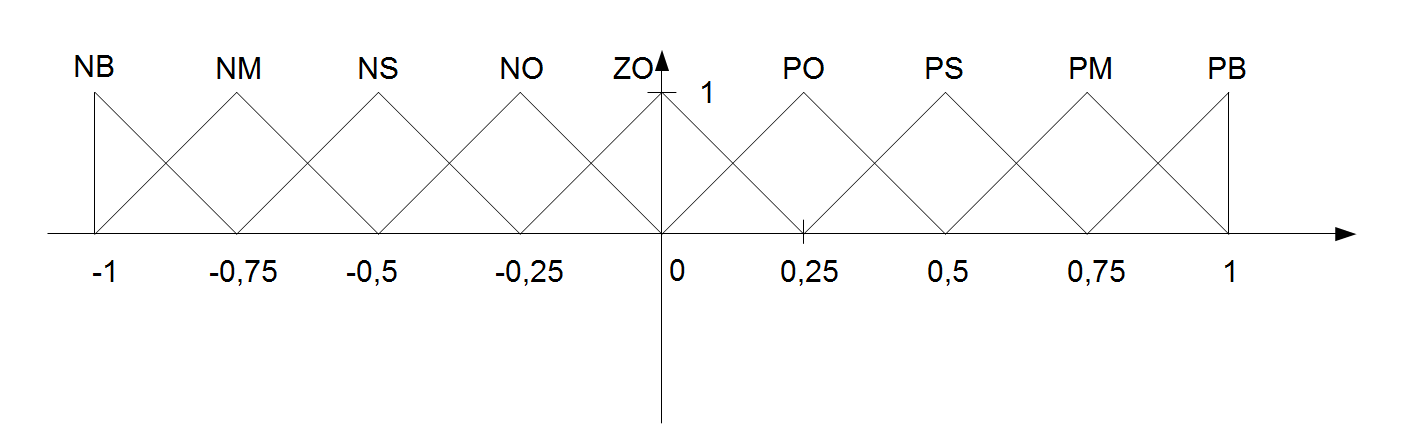
\includegraphics[scale=0.5]{pics/explode.png}
\caption{Разбиение универсального множества}
\label{fig.2}
\end{figure}

В соответствии с вышеприведенным графиком получим следующие треугольные числа:

\begin{itemize}
\item <<NB>> $\left(-1;0;0,25\right)$;
\item <<NM>> $\left(-0,75;0,25;0,25\right)$;
\item <<NS>> $\left(-0,5;0,25;0,25\right)$;
\item <<NO>> $\left(-0,5;0,25;0,25\right)$;
\item <<ZO>> $\left(0;0,25;0,25\right)$;
\item <<PO>> $\left(0,25;0,25;0,25\right)$;
\item <<PS>> $\left(0,5;0,25;0,25\right)$;
\item <<PM>> $\left(0,75;0,25;0,25\right)$;
\item <<PB>> $\left(1;0,25;0\right)$.
\end{itemize}

На основании этих оценок мы можем установить общую тональность лингвистической единицы $S_i$.

В качестве общего массива данных выступают:
\begin{itemize}
\item $S_i$~--- тональная оценка лексической единицы, $i=\overline{1,N}$, где $N$~--- количество слов базового словаря;
\item $s_{ij}$~--- оценка $S_i$ экспертом $j$, $j=\overline{1,k_i}$, где $k_i$~--- количество оценок $S_i$.
\end{itemize}

\subsection{Медиана лингвистических переменных}

Определение медианы согласно :
%\begin{Def}
Определение. Медиана~-- значение некоторого признака (варианта), приходящееся на средину ранжированной (упорядоченной) совокупности, т.~е. элемент, делящий некоторое множество на две равные по объему количества элементов части.
%\end{Def}

Медиана не зависит от крайних значений или выбросов (т.~е. является проявляет более сильную робастность), при этом являясь одним из методов центрирования некоторого распределения. В дискретных рядах (в данном случае) медиана находится непосредственно по накопленной частоте, соответствующей номеру медианы.

\subsection{Операции с лингвистическими переменными}

Из определения медианы явно следует, что перед вычислением самой медианы некоторая последовательность должна быть проранжирована, т.~е. упорядочена. В частности, это значит, что для проведения данной процедуры для элементов множества должны быть определены следующие операции (отношения строгого порядка):
\begin{itemize}
\item больше $\left(>\right)$;
\item меньше $\left(<\right)$;
\item равно $\left(=\right)$;
\item не равно $\left(\neq\right)$.
\end{itemize}

Данные операции и их производные $\left(\leq,\geq\right)$ используются во всех известных (7 видов) алгоритмах сравнения, включая ответвления для различных мощностей входных данных.

Указанные операции определены для множества действительных чисел $\mathbb{R}$, однако в случае лингвистических переменных требуют пояснения.
\subsubsection{Операции <<равно>>, <<не равно>>}

Пусть даны два треугольных числа: $T_1\left(a_1,\gamma_1,\delta_1\right)$ и $T_2\left(a_2,\gamma_2,\delta_2\right)$. Требуется определить операции <<равно>>, <<не равно>> аналогично множеству действительных чисел.

Учитывая то, что треугольное число определяется тройкой действительных, требуемые операции определяются тривиально:

%\begin{Def}
Определение. Считать равными два треугольных числа $T_1$ и $T_2$, если их числовые характеристики $a, \gamma$ и $\delta$ соответственно равны между собой (т.~е. $a_1=a_2, \gamma_1=\gamma_2, \delta_1=\delta_2$), иначе считать числа $T_1$ и $T_2$ не равными между собой.
%\end{Def}

\subsubsection{Операции <<меньше>>, <<больше>>}

Для определения данного вида отношений не могут быть использованы столь же тривиальные правила, как для отношений <<равно>>, <<не равно>>.

Для определения операций над нечеткими числами существует два способа: использование $\alpha$-сечения или использование принципа расширения Заде. Опишем использование $\alpha$-сечения.

%\begin{Def}
Определение. $\alpha$-сечением (или $\alpha$-уровнем, срезом, уровневым представлением) $\left[A\right]^\alpha$ нечеткого числа $A\in\mathcal{F}$ называется множество

$$
\left\{
\begin{aligned}
\left\{t\in R\vert\mu\left(t\right)\geq\alpha\right\}, & \text{ если } \alpha > 0; \\
\overline{supp\left(A\right)}, & \text{ если } \alpha = 0;
\end{aligned}
\right.
$$

где $supp\left(A\right)$~-- замыкание некоторого нечеткого множества, т.~е. при $supp\left(A\right)=\left(a, b\right)$ нулевым уровнем будет $\left[a,b\right]$.
%\end{Def}

Нечеткое число обычно определяется набором $\alpha$-сечений, при заданном наборе значений $\left\{\alpha\right\}$. Для треугольного числа достаточно определить два $\alpha$-сечения (при $\alpha=0$ и $\alpha=1$), остальные выводятся из них.

Представим два треугольных числа $T_1$ и $T_2$ в уровневой форме, тогда будем иметь:

$$
\begin{aligned}
{T_1}_{\stackrel{'}I}\Leftrightarrow & \left({T_1}_{\stackrel{'}I}\left(\mu\right),\overline{{T_1}_{\stackrel{'}I}}\left(\mu\right)\right), 0\leq\mu\leq 1 \\
{T_2}_{\stackrel{'}I}\Leftrightarrow & \left({T_2}_{\stackrel{'}I}\left(\mu\right),\overline{{T_2}_{\stackrel{'}I}}\left(\mu\right)\right), 0\leq\mu\leq 1
\end{aligned}
$$

где $\Leftrightarrow$~-- символ эквивалентности.

Для $T_1$ и $T_2$ введем критерии:

$$
\begin{aligned}
R_1 &= \int\limits_0^1 \mu\cdot\left[{T_1}_{\stackrel{'}I}\left(\mu\right)+\overline{{T_1}_{\stackrel{'}I}}\left(\mu\right)\right] d\mu \\
R_2 &= \int\limits_0^1 \mu\cdot\left[{T_2}_{\stackrel{'}I}\left(\mu\right)+\overline{{T_2}_{\stackrel{'}I}}\left(\mu\right)\right] d\mu
\end{aligned}
$$

Для данных критериев, если $R_1<R_2$, то $T_1<T_2$, т.~е., интегрируя и получая на выходе действительные числа, проводим над ними уже определенные операции упорядочивания.

Можно показать, что введенное отношение является транзитивным и рефлексивным, т.~е. для некоторого бинарного отношения $K$:
\begin{itemize}
\item транзитивность $K$: для $T_1,T_2$ и $T_3$, если $T_1 K T_2$ и $T_2 K T_3$, то и $T_1 K T_3$;
\item рефлексивность $K$: если $T K T \forall T\subset \mathcal{F}$
\end{itemize}

Если расписать данное отношение применительно к обозначению $\left(a,\gamma,\delta\right)$ некоторого треугольного числа $T$, то получим, что критерий $R$ вычисляется по формуле:

$$
R=\int\limits_0^1 x\cdot\left(\gamma\cdot x+a-\gamma\right)\cdot\left(a+\delta-\delta\cdot x\right) dx
$$

Учитывая многочисленные методы численного интегрирования, ранжирование треугольных чисел благодаря данному мат.~аппарату становится тривиальной задачей.
\section{Определение тональности текста}
\subsection{Аннотирование}

Формируемые системой аннотации должны удовлетворять ряду требований. Их можно разделить на требования, которые выдвигает пользователь, и требования, которые накладываются реализацией системы. Можно назвать следующие требования, выдвигаемые пользователем:

\begin{enumerate}
\item Аннотация должна давать представление о том, какую информацию содержит документ о предмете запроса;
\item Быть достаточно короткой, чтобы ее анализ пользователем не занимал много времени. Человек должен иметь возможность охватить сформированный текст <<одним взглядом>>;
\item В случае большого документа, она должна давать представление о том, какие части документа несут релевантную информацию.
\end{enumerate}

При аннотации больших документов следует использовать разметку документа для разбиения его на несколько аннотируемых частей.

Ниже описаны применяемые алгоритмы реализации аннотирования.

\subsubsection{Базовый алгоритм}

Рекомендуемое значение аннотируемой единицы находится в пределе 35 синтаксических единиц или 300 символов. Вес фрагмента определяется по следующей формуле:

$$
	W_b=\sum\limits_{i=1}^n w_i + \dfrac{Kn}{L}
$$

где $\sum\limits_{i=1}^n w_i$~--- сумма весов синтаксических единиц запроса, вошедших в фрагмент. Каждое слово учитывалось только один раз. Вес каждого слова зависел от распределения слова в коллекции и был тем выше, чем более редкое это слово. Он рассчитывался по формуле:

$$
	w_i = \dfrac{\log_2\left(N_i\right)}{\log_2\left(N\right)}
$$

$K$~--- некоторая константа;

$n$~--- число слов из запроса, которые встретились во фрагменте;

$L$~--- расстояние между первым и последним словом запроса, встретившимся во фрагменте.

\subsubsection{Алгоритм Freq}

Данный алгоритм проводит анализ блока примерно в 1000 слов вокруг целевого фрагмента. Отбираются 10 слов, которые встречаются в данном фрагменте наиболее часто.

$$
	W_{freq}=W_b+\sum\log_2\left(F_k\right)
$$

где $W_b$~--- вес, вычисленный по базовому алгоритму, $F_k$~--- количество вхождений слова в окне из 1000 слов.

\subsubsection{Алгоритм LRU-K}

Реализация следующая:

\begin{enumerate}
\item Создаются 3 структуры данных: массивы слов и 2 массива с указателями на слова ($a_1$ и $a_2$ соответственно).
\item Для каждого слова при обработке документа производились следующие действия
\begin{enumerate}
\item Если слово не найдено, то ссылка на него помещается в массив $a_1$ в первую позицию, остальные позиции в массиве сдвигаются, самое последнее слово удаляется из $a_1$ и из массива слов;
\item Если слово найдено и встречается в $a_1$, то оно из него удаляется и переносится на первую позицию в $a_2$. При этом, если $a_2$ полностью заполнен, то последнее слово из него так же удаляется, как и в первом случае.
\item Если слово найдено и уже было в $a_2$, то оно просто перемещается на первую позицию.
\end{enumerate}
\end{enumerate}

Вычисление веса фрагмента производится по алгоритму Freq.

\subsection{Оценка тональности}

Для оценки тональности текста $P$ производится подсчет суммы тональностей аннотированных синтаксических единиц текста, учитывая их вес:

$$
P=\sum\limits_i TR\left(i\right)\cdot Q\left(i\right)
$$

\section{Выводы}

В данной части последовательно рассмотрены основные типы задач, которые требуется решить для анализа тональности информационного поля. Приведен основной алгоритм, подобрана и приведена математическая формализация каждого из его пунктов, дано обоснование использования приведенных моделей. Освещена проблема реализуемости каждого этапа.

Для синтаксического анализа проработаны модели, определяющая математическое представление некоторого предложения, рассмотрены их основные достоинства и недостатки. Предложена наиболее оптимальная с точки зрения адекватности поставленной задаче.

Для оценки тональности некоторой лексической единицы, используя положения нечеткой логики, сформирован математический аппарат, позволяющий тривиальным образом решить задачу, опираясь на основные положения математической статистики. Определены формулы, предоставляющие базис для решения не только данной подзадачи, но и более широкого класса задач в перспективе.

Подробно рассмотрены основные алгоритмы аннотирования текста, приведено обоснование выбора единицы аннотирования. Выбран наиболее оптимальный с точки зрения получаемых результатов алгоритм аннотирования.

Ясно видно, что решение данной задачи обосновано только при применении данных разработок в конечном программном продукте, в связи с чем и было разработано приложение, способное выполнять весь спектр требуемых задач по анализу тональности информационного поля.
\newpage
\chapter{Программная реализация}
\section{Описание программы}
\subsection{Общие сведения}

Название программного комплекса: Оценка тональности информационного поля.

Исполняемый файл: fiver

Программа разработана в IDE Qt Creator, на языке программирования С++, диалект Qt.

\subsection{Функциональное назначние}

Программа <<Оценка тональности информационного поля>> предназначена для анализа информационной тональности документа(-ов) относительно некоторого термина. Для определения информационной тональности использован математический аппарат нечеткой логики, теории графов, математической статистики, логики предикатов, линейной алгебры, методов оптимизации, что позволяет оценить тональность того или иного документа относительно мнения пользователя.

\subsection{Описание логической структуры}

Программный комплекс представляет собой следующий набор файлов и модулей:

\begin{enumerate}
\item fiver. Основной исполняемый файл программы. Для него должны быть установлены права на исполнение от лица запускающего пользователя.
\item Модули Qt 5, представленые следующим набором:
\begin{enumerate}
\item Qt 5 Gui, пользовательский интерфейс;
\item Qt 5 Core, основные примитивы;
\item Qt 5 Network, работа с сетью;
\item Qt 5 Xml, работа с XML.
\end{enumerate}
\item Модули библиотеки Boost, представленные следующим набором
\begin{enumerate}
\item Boost.Thread, создание и управление потоками приложения;
\item Boost.System, системные примитивы, требуется для модуля Boost.Thread
\item Boost.Regex, регулярные выражения.
\end{enumerate}
\item Библиотека GSL, реализующая большинство математических операций над данными;
\item Библиотека o2scl, являющаяся объектно-ориентированной оберткой над GSL и предоставляющая упрощенный доступ, в частности, к возможностям численного интегрирования.
\item Комплекс solarix, предназначенный для синтаксического и морфологического анализов.
\end{enumerate}

Также требуется настроенная СУБД MySQL, с базой данных специального формата (формат будет описан далее).

Невозможность компоновки всего в единый файл определена как используемыми данными библиотеками лицензиями (в частности, Qt имеет, помимо свободной, еще и проприетарную лицензию), так и неразумностью данного шага, так как все библиотеки могут быть установлены из официальных репозиториев любого Linux-дистрибутива.

Для взаимодействия с пользователем программа дружественный интерфейс пользователя. Формы, меню и части программы взаимодействуют межу собой и ОС посредством механизма сигналов и слотов. Программа разработана с помощью IDE Qt Creator.

Программа содержит основную форму <<mainwindow.ui>>, скомпонированную в странично-ориентированном виде, т.~е. определенная задача, выполняемая программой, представлена как отдельная страница, вызываемая по запросу.

Также программа представлена следующими формами:

\begin{itemize}
\item <<aboutdialog.ui>>~-- диалог данных <<О программе...>>;
\item <<appenduridialog.ui>>~-- диалог добавления нового URL документа для анализа;
\item <<changemarkdialog.ui>>~-- диалог смены оценки для элемента словаря;
\item <<insertarticledialog.ui>>~-- диалог для добавления новой словарной статьи в БД;
\item <<optionsdialog.ui>>~-- диалог для определения настроек программы (соединение с БД и файл словаря размеченного корпуса русского языка, используемый при синтаксическом и морфологическом анализах).
\end{itemize}

Для каждой формы определен соответствующий ей класс,  позволяющий взаимодействовать с остальными компонентами приложения. В общем виде UML-диаграмма классов такова:

\begin{figure}[h]
\centering
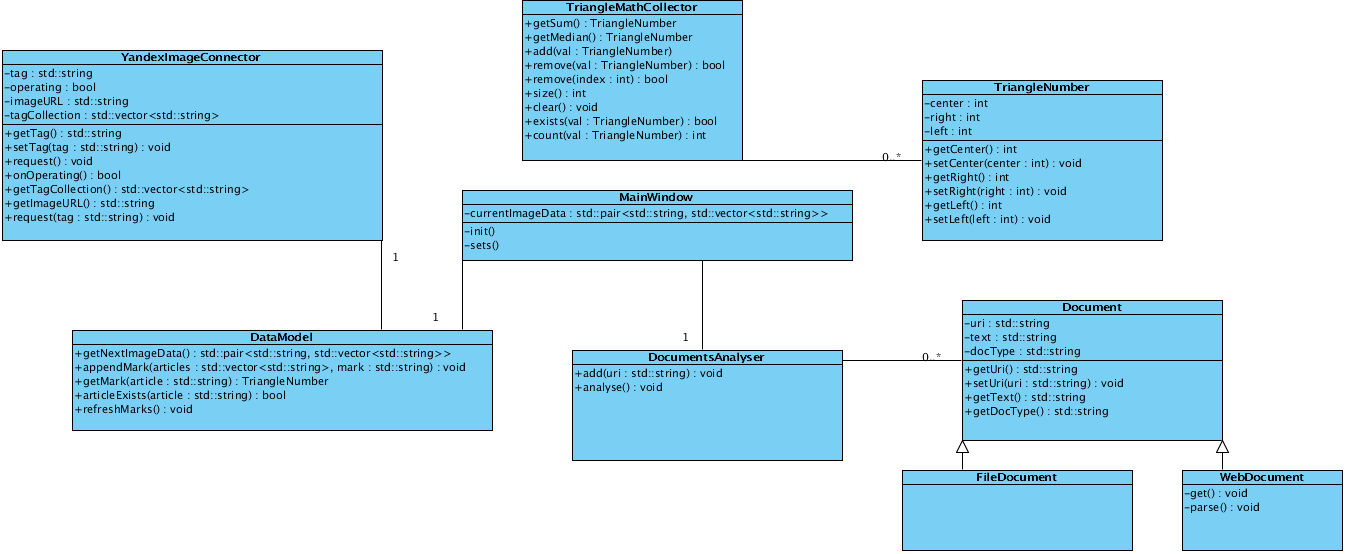
\includegraphics[scale=0.45]{pics/class.png}
\caption{Диаграмма классов}
\label{fig.0}
\end{figure}

Перечислим основные классы и их функции (алфавитный порядок).

\subsubsection{Класс AboutDialog}

Наследуется от: QDialog
Назначение: описание диалога <<О программе...>>

\subsubsection{Класс AppendUriDialog}

Наследуется от: QDialog

Назначение: описание диалога добавления нового URL в список анализируемых.

\begin{longtable}{|m{3 cm}|m{3 cm}|m{4 cm}|m{4 cm}|}
\caption{Методы класса AppendUriDialog\label{tab:appenduridlg}} \\
\hline 
Имя метода & Описание & Входные параметры & Выходные параметры \\
\hline
\endfirsthead
\caption*{Продолжение таблицы \ref{tab:appenduridlg}} \\
\hline
Имя метода & Описание & Входные параметры & Выходные параметры \\
\endhead
getUri & Возвращает введенный в поле URL & void & QString~-- URL \\
\hline
getExpertMark & Возвращает пользовательскую экспертную оценку & void & int~-- целочисленный идентификатор оценки \\
\hline
clear & Очистка входных данных & void & void \\
\hline 
\end{longtable}

\subsubsection{Класс CategoryMaster}

Назначение: содержит некоторые константы, используемые в приложении повсеместно.

\subsubsection{Класс ChangeMarkDialog}

Наследуется от: QDialog

Назначение: описание диалога изменения оценки статьи.

\begin{longtable}{|m{3 cm}|m{3 cm}|m{4 cm}|m{4 cm}|}
\caption{Методы класса ChangeMarkDialog\label{tab:changemarkdlg}} \\
\hline 
Имя метода & Описание & Входные параметры & Выходные параметры \\
\hline
\endfirsthead
\caption*{Продолжение таблицы \ref{tab:changemarkdlg}} \\
\hline
Имя метода & Описание & Входные параметры & Выходные параметры \\
\endhead
init & Метод инициализации & void & void \\
\hline
sets & Метод, выполняющий предустановки & void & void \\
\hline
conn & Метод, выполняющий сигнально-слотовые соединения & void & void \\
\hline
getVoteMark & Извлекает установленную оценку & void & int~-- целочисленный идентификатор оценки \\
\hline
{voteValue\-Changed} & Применяется для установки значения текста кнопки в зависимости от числового идентификатора & int~-- целочисленный идентификатор оценки & void \\
\hline
\end{longtable}

\subsubsection{Класс DataModel}

Наследуется от: QObject

Назначение: один из основных классов. Используется преимущественно для доступа к базе данных и извлечения из нее необходимой информации. Также генерирует основные наборы данных.

\begin{longtable}{|m{3 cm}|m{3 cm}|m{4 cm}|m{4 cm}|}
\caption{Методы класса DataModel\label{tab:datamodel}} \\
\hline 
Имя метода & Описание & Входные параметры & Выходные параметры \\
\hline
\endfirsthead
\caption*{Продолжение таблицы \ref{tab:datamodel}} \\
\hline
Имя метода & Описание & Входные параметры & Выходные параметры \\
\endhead
init & Метод инициализации & void & void \\
\hline
sets & Метод, выполняющий предустановки & void & void \\
\hline
conn & Метод, выполняющий сигнально-слотовые соединения & void & void \\
\hline
{getNext\-ImageData} & Возвращает новые данные для заполнения (теги и ссылку на тематическое изображение) & void & std::pair~-- пара, первый элемент которой (std::string)~-- строка (ссылка на изображение), второй~-- вектор строк (теги) \\
\hline
appendMark & Устанавливает оценку для набора статей & void & void \\
\hline
getMark & Возвращает оценку для статьи классом треугольного числа & std::string~-- имя статьи & TriangleNumber~-- оценка \\
\hline
articleExists & Проверка существования статьи & std::string~-- имя статьи & bool~-- true если статья существует, иначе false \\
\hline
refreshMarks & Обновление оценок в словаре & void & void \\
\hline
{getMain\-Window} & Извлечение указателя на главное окно & void & MainWindow*~-- указатель на главное окно \\
\hline
{setMain\-Window} & Установка указателя на главное окно & MainWindow*~-- указатель на главное окно & void \\
\hline
{getNext\-RandomTag} & Запускает цикл поиска случайного тега в БД & void & void \\
\hline
{dbLink\-IsCorrect} & Проверка соединения базой данных & void & bool~-- true если соединение с БД корректно, иначе false \\
\hline
getHost & Возвращает адрес сервера БД & void & QString~-- адрес сервера БД \\
\hline
setHost & Установка адреса сервера БД & QString~-- адрес сервера БД & void \\
\hline
{get\-Username} & Возвращает имя пользователя БД & void & QString~-- имя пользователя \\
\hline
{set\-Username} & Устанавливает имя пользователя БД & QString~-- имя пользователя & void \\
\hline
getPass & Возвращает пароль БД & void & QString~-- пароль БД \\
\hline
setPass & Устанавливает пароль БД & QString~-- пароль БД & void \\
\hline
{getDb\-Name} & Возвращает имя базы данных & void & QString~-- имя БД \\
\hline
{setDb\-Name} & Устанавливает имя базы данных & QString~-- имя БД & void \\
\hline
getPort & Возвращает порт соединения с БД & void & int~-- номер порта \\
\hline
setPort & Устанавливает порт соединения с БД & int~-- номер порта & void \\
\hline
{get\-Map\-Table\-Model} & Возвращает модель БД & void & {QSql\-Table\-Model*}~-- модель БД \\
\hline
{set\-Map\-Table\-Model} & Устанавливает модель БД & {QSql\-Table\-Model*}~-- модель БД & void \\
\hline
{get\-Map\-Row\-Count} & Возвращает количество статей в словаре & void & int~-- количество статей в словаре \\
\hline
{set\-Map\-Row\-Count} & Возвращает количество статей в словаре & int~-- количество статей в словаре & void \\
\hline
{conn\-Main\-Window} & Сигнально-слотовые соединения с главным окном & void & void \\
\hline
{create\-Model} & Создание модели БД & void & void \\
\hline
{rebuild\-Limits\-Distribution} & Перестроение генерации случайного распределения & void & void \\
\hline
\end{longtable}

Используемые слоты:

\begin{longtable}{|m{3 cm}|m{3 cm}|m{4 cm}|m{4 cm}|}
\caption{Слоты класса DataModel\label{tab:datamodelsl}} \\
\hline 
Имя метода & Описание & Входные параметры & Выходные параметры \\
\hline
\endfirsthead
\caption*{Продолжение таблицы \ref{tab:datamodelsl}} \\
\hline
Имя метода & Описание & Входные параметры & Выходные параметры \\
\endhead
{on\-Image\-Info\-Loaded} & Вызывается при загрузке данных & void & void \\
\hline
{load\-Image\-Info} & Загрузка набора данных & void & void \\
\hline
reconn & Выполняет пересоединение с базой данных & void & void \\
\hline
{options\-Accepted} & Опции установлены & void & void \\
\hline
{options\-Rejected} & Опции отклонены & void & void \\
\hline
{load\-Image\-Info\-Loop} & Запускает петлю запросов & bool~-- true, если предыдущий запрос завершился удачно, иначе false & void \\
\hline
{on\-Tag\-Loaded} & Вызывается при загрузке тега & QString~-- тег & void \\
\hline
\end{longtable}

Используемые сигналы:

\begin{longtable}{|m{3 cm}|m{3 cm}|m{4 cm}|m{4 cm}|}
\caption{Сигналы класса DataModel\label{tab:datamodelsig}} \\
\hline 
Имя метода & Описание & Входные параметры & Выходные параметры \\
\hline
\endfirsthead
\caption*{Продолжение таблицы \ref{tab:datamodelsig}} \\
\hline
Имя метода & Описание & Входные параметры & Выходные параметры \\
\endhead
{image\-Info\-Loaded} & Отправляется при загрузке изображения & void & void \\
\hline
{recieve\-Info} & Отправка информации об ошибке & {Errors::Img\-Error\-Code}~-- код ошибки, QString~-- сообщение об ошибке & void \\
\hline
{db\-Connected\-Status} & Проверка доступа к БД & bool~-- true если соединение с БД установлено и корректно, иначе false & void \\
\hline
{load\-This\-Tag} & Просит загрузить тег & QString~-- тег & void \\
\hline
\end{longtable}

\subsubsection{Класс Document}

Наследуется от: QObject, CategoryMaster

Назначение: абстракция анализируемого документа. Производит чтение документа из ресурса и предварительный парсинг.

\begin{longtable}{|m{3 cm}|m{3 cm}|m{4 cm}|m{4 cm}|}
\caption{Методы класса Document\label{tab:document}} \\
\hline 
Имя метода & Описание & Входные параметры & Выходные параметры \\
\hline
\endfirsthead
\caption*{Продолжение таблицы \ref{tab:document}} \\
\hline
Имя метода & Описание & Входные параметры & Выходные параметры \\
\endhead
init & Метод инициализации & void & void \\
\hline
getUri & Возвращает URL ресурса & void & QString~-- URL \\
\hline
setUri & Устанавливает URL ресурса & QString~-- URL & void \\
\hline
{get\-Doc\-Type} & Возвращает тип документа & void & QString~-- тип документа \\
\hline
{get\-State} & Возвращает значение состояния анализа документа & void & {Document\-State::\-Processing\-State}~-- состояние процесса \\
\hline
{set\-State} & Устанавливает значение состояния анализа документа & {Document\-State::\-Processing\-State}~-- состояние процесса & void \\
\hline
{get\-Grammar\-Engine} & Возвращает дескриптор грамматического движка & void & HGREN~-- дескриптор движка \\
\hline
{set\-Grammar\-Engine} & Устанавливает дескриптор грамматического движка & HGREN~-- дескриптор движка & void \\
\hline
{get\-Lemmas} & Возвращает предложения документа & void & Вектор QString~-- набор предложений \\
\hline
{set\-Lemmas} & Устанавливает предложения документа & Вектор QString~-- набор предложений & void \\
\hline
\end{longtable}

Чисто виртуальные методы:

\begin{longtable}{|m{3 cm}|m{3 cm}|m{4 cm}|m{4 cm}|}
\caption{Чисто виртуальные методы класса Document\label{tab:documentvirt}} \\
\hline 
Имя метода & Описание & Входные параметры & Выходные параметры \\
\hline
\endfirsthead
\caption*{Продолжение таблицы \ref{tab:documentvirt}} \\
\hline
Имя метода & Описание & Входные параметры & Выходные параметры \\
\endhead
sets & Метод, выполняющий предустановки & void & void \\
\hline
conn & Метод, выполняющий сигнально-слотовые соединения & void & void \\
\hline
{prepare\-Text} & Выполняет подготовку текста для синтаксического разбора & void & void \\
\hline
{refresh\-Tone} & Вычисление тональности документа & void & void \\
\hline
\end{longtable}

Используемые сигналы:

\begin{longtable}{|m{3 cm}|m{3 cm}|m{4 cm}|m{4 cm}|}
\caption{Сигналы класса Document\label{tab:documentsig}} \\
\hline 
Имя метода & Описание & Входные параметры & Выходные параметры \\
\hline
\endfirsthead
\caption*{Продолжение таблицы \ref{tab:documentsig}} \\
\hline
Имя метода & Описание & Входные параметры & Выходные параметры \\
\endhead
{percent\-Completed} & Процентное выполнение задачи & int~-- процент & void \\
\hline
message & Сообщение & QString~-- содержание сообщения & void \\
\hline
{send\-Tone} & Отправка текущей определенной тональности документа & QString~-- тональность & void \\
\hline
{try\-Set\-Info} & Попытка отправить информацию в нужную колонку & int~-- номер колонки, QString~-- строка & void \\
\hline
{text\-Prepared} & Подготовка текста окончена & void & void \\
\hline
\end{longtable}

\subsubsection{Класс DocumentsAnalyser}

Наследуется от: QObject

Назначение: Анализирует эмоциональную тональность набора документов.

\begin{longtable}{|m{3 cm}|m{3 cm}|m{4 cm}|m{4 cm}|}
\caption{Методы класса DocumentsAnalyser\label{tab:documentanalyser}} \\
\hline 
Имя метода & Описание & Входные параметры & Выходные параметры \\
\hline
\endfirsthead
\caption*{Продолжение таблицы \ref{tab:documentanalyser}} \\
\hline
Имя метода & Описание & Входные параметры & Выходные параметры \\
\endhead
init & Метод, выполняющий предварительную инициализацию & void & void \\
\hline
sets & Метод, выполняющий предустановки & void & void \\
\hline
conn & Метод, выполняющий сигнально-слотовые соединения & void & void \\
\hline
add & Добавляет ресурс для анализа & std::string~-- имя ресурса, int~-- экспертная оценка & bool~-- true, если URL корректен, иначе false \\
\hline
{get\-Resourse\-List\-Model} & Возвращает модель данных для отображения & void & {QStandard\-Item\-Model}~-- модель данных \\
\hline
{set\-Resourse\-List\-Model} & Устанавливает модель данных для отображения & {QStandard\-Item\-Model}~-- модель данных & void \\
\hline
{remove\-Row} & Удаляет выбранный ресурс & void & void \\
\hline
{get\-Termine} & Возвращает значение анализируемого термина & void & QString~-- термин \\
\hline
{get\-DBModel} & Возвращает модель БД & void & {Data\-Model*}~-- модель БД \\
\hline
{set\-DBModel} & Устанавливает модель БД & {Data\-Model*}~-- модель БД & void \\
\hline
{reload\-Gramma\-Engine} & Перезагрузка грамматического движка & void & void \\
\hline
\end{longtable}

Используемые слоты:
\begin{longtable}{|m{3 cm}|m{3 cm}|m{4 cm}|m{4 cm}|}
\caption{Слоты класса DocumentsAnalyser\label{tab:documentanalysersl}} \\
\hline 
Имя метода & Описание & Входные параметры & Выходные параметры \\
\hline
\endfirsthead
\caption*{Продолжение таблицы \ref{tab:documentanalysersl}} \\
\hline
Имя метода & Описание & Входные параметры & Выходные параметры \\
\endhead
{doc\-Text\-Prepared} & Документ закончил подготовку текста & void & void \\
\hline
{doc\-Percent\-Completed} & Документ провел некоторую часть работ & int~-- процент & void \\
\hline
{doc\-Message} & Документ послал сообщение & QString~-- текст сообщения & void \\
\hline
{recieve\-Column} & Документ просит установить значение в колонку & int~-- номер колонки, QString~-- значение & void \\
\hline
{doc\-Tone} & Установка тональности & QString~-- тональность & void \\
\hline
\end{longtable}

Используемые сигналы:
\begin{longtable}{|m{3 cm}|m{3 cm}|m{4 cm}|m{4 cm}|}
\caption{Сигналы класса DocumentsAnalyser\label{tab:documentanalysersig}} \\
\hline 
Имя метода & Описание & Входные параметры & Выходные параметры \\
\hline
\endfirsthead
\caption*{Продолжение таблицы \ref{tab:documentanalysersig}} \\
\hline
Имя метода & Описание & Входные параметры & Выходные параметры \\
\endhead
error & Ошибка & QString~-- сообщение & void \\
\hline
\end{longtable}

\subsubsection{Класс MainWindow}

Наследуется от: QMainWindow, CategoryMaster

Назначение: описывает главное окно; также выполняет связующие функции для остальных объектов.

\begin{longtable}{|m{3 cm}|m{3 cm}|m{4 cm}|m{4 cm}|}
\caption{Методы класса MainWindow\label{tab:mainwindow}} \\
\hline 
Имя метода & Описание & Входные параметры & Выходные параметры \\
\hline
\endfirsthead
\caption*{Продолжение таблицы \ref{tab:mainwindow}} \\
\hline
Имя метода & Описание & Входные параметры & Выходные параметры \\
\endhead
init & Метод, выполняющий предварительную инициализацию & void & void \\
\hline
sets & Метод, выполняющий предустановки & void & void \\
\hline
conn & Метод, выполняющий сигнально-слотовые соединения & void & void \\
\hline
{resize\-Event} & Изменение размера окна & {QResize\-Event*}~-- событие изменения & void \\
\hline
{get\-Current\-Mark} & Возвращает текущую оценку & int~-- численный идентификатор оценки & void \\
\hline
{image\-Resize} & Изменение размера загруженного изображения & void & void \\
\hline
\end{longtable}

Используемые слоты:

\begin{longtable}{|m{3 cm}|m{3 cm}|m{4 cm}|m{4 cm}|}
\caption{Слоты класса MainWindow\label{tab:mainwindowsl}} \\
\hline 
Имя метода & Описание & Входные параметры & Выходные параметры \\
\hline
\endfirsthead
\caption*{Продолжение таблицы \ref{tab:mainwindowsl}} \\
\hline
Имя метода & Описание & Входные параметры & Выходные параметры \\
\endhead
{recieve\-Message} & Принимает сообщение & {Errors::Img\-Error\-Code}~-- код сообщения, QString~-- строка сообщения & void \\
\hline
{download\-Progress} & Отслеживает состояние загрузки ресурсов & qint64~-- байт загружено, qint64~-- байт всего & void \\
\hline
{state\-Changed} & Вызывается при смене настроек & void & void \\
\hline
{recieve\-Error} & Принимает сообщение об ошибке & QString~-- текст сообщения & void \\
\hline
{voc\-Action\-Performed} & Выбор действия для словаря & void & void \\
\hline
{tone\-Action\-Performed} & Выбор действия для оценки тональностей & void & void \\
\hline
{load\-Image} & Загрузка изображения & void & void \\
\hline
{image\-Loaded} & Отображение изображения & {QNetwork\-Reply*}~-- ответ сервера & void \\
\hline
dbCheck & Проверка соединения с БД & bool~-- true, если соединение установлено, иначе false & void \\
\hline
{vote\-Val\-Changed} & Установка слайдера оценки & int~-- численный код оценки & void \\
\hline
{operation\-Change} & Смена отображаемого виджета & int~-- индекс стекового виджета & void \\
\hline
{remove\-Selected\-Data} & Удаление текущей выделенной строки & void & void \\
\hline
{append\-Data\-After\-Current} & Вставка новой строки & void & void \\
\hline
{change\-Vote\-Mark} & Процедура изменения оценки статьи & void & void \\
\hline
{append\-New\-Uri} & Процедура добавления нового URL & void & void \\
\hline
{remove\-Resourse\-Row} & Процедура удаления строки & void & void \\
\hline
{open\-Help} & Открыть справку & void & void \\
\hline
\end{longtable}

\subsubsection{Класс OptionsDialog}

Наследуется от: QDialog

Назначение: описывает диалог настроек программы

\begin{longtable}{|m{3 cm}|m{3 cm}|m{4 cm}|m{4 cm}|}
\caption{Методы класса OptionsDialog\label{tab:optionsdialog}} \\
\hline 
Имя метода & Описание & Входные параметры & Выходные параметры \\
\hline
\endfirsthead
\caption*{Продолжение таблицы \ref{tab:optionsdialog}} \\
\hline
Имя метода & Описание & Входные параметры & Выходные параметры \\
\endhead
init & Метод, выполняющий предварительную инициализацию & void & void \\
\hline
sets & Метод, выполняющий предустановки & void & void \\
\hline
conn & Метод, выполняющий сигнально-слотовые соединения & void & void \\
\hline
getHost & Возвращает адрес сервера БД & void & QString~-- адрес сервера БД \\
\hline
setHost & Установка адреса сервера БД & QString~-- адрес сервера БД & void \\
\hline
{get\-Username} & Возвращает имя пользователя БД & void & QString~-- имя пользователя \\
\hline
{set\-Username} & Устанавливает имя пользователя БД & QString~-- имя пользователя & void \\
\hline
getPass & Возвращает пароль БД & void & QString~-- пароль БД \\
\hline
setPass & Устанавливает пароль БД & QString~-- пароль БД & void \\
\hline
{getDb\-Name} & Возвращает имя базы данных & void & QString~-- имя БД \\
\hline
{setDb\-Name} & Устанавливает имя базы данных & QString~-- имя БД & void \\
\hline
getPort & Возвращает порт соединения с БД & void & int~-- номер порта \\
\hline
setPort & Устанавливает порт соединения с БД & int~-- номер порта & void \\
\hline
{get\-Dict\-Path} & Возвращает путь к файлу словаря & void & QString~-- путь \\
\hline
{get\-Dict\-Path} & Устанавливает путь к файлу словаря & QString~-- путь & void \\
\hline
\end{longtable}

Используемые слоты:

\begin{longtable}{|m{3 cm}|m{3 cm}|m{4 cm}|m{4 cm}|}
\caption{Слоты класса OptionsDialog\label{tab:optionsdialogsl}} \\
\hline 
Имя метода & Описание & Входные параметры & Выходные параметры \\
\hline
\endfirsthead
\caption*{Продолжение таблицы \ref{tab:optionsdialogsl}} \\
\hline
Имя метода & Описание & Входные параметры & Выходные параметры \\
\endhead
{choose\-Dict\-Path} & Выбор расположения файла словаря & void & void \\
\hline
load & Загрузка настроек & void & void \\
\hline
save & Сохранение настроек & void & void \\
\hline
\end{longtable}

\subsubsection{Класс TriangleMathCollector}

Назначение: Класс реализует арифметику для треугольных чисел.

\begin{longtable}{|m{3 cm}|m{3 cm}|m{4 cm}|m{4 cm}|}
\caption{Методы класса TriangleMathCollector\label{tab:trianglemathcollector}} \\
\hline 
Имя метода & Описание & Входные параметры & Выходные параметры \\
\hline
\endfirsthead
\caption*{Продолжение таблицы \ref{tab:trianglemathcollector}} \\
\hline
Имя метода & Описание & Входные параметры & Выходные параметры \\
\endhead
getSum & Возвращает сумму треугольных чисел в коллекторе & void & {Triangle\-Number}~-- сумма \\
\hline
{get\-Median} & Возвращает медиану треугольных чисел в коллекторе & void & {Triangle\-Number}~-- значение медианы \\
\hline
add & Добавляет треугольное число в коллектор & {Triangle\-Number}~--треугольное число & void \\
\hline
size & Возвращает размер коллектора & void & int~-- размер коллектора \\
\hline
clear & Очищает коллектор & void & void \\
\hline
exists & Определяет, присутствует ли данное треугольное число в коллекторе & {Triangle\-Number}~--треугольное число & bool~-- true если присутствует, иначе false \\
\hline
count & Подсчитывает количество чисел в коллекторе & {Triangle\-Number}~--треугольное число & int~-- количество вхождений числа в коллектор \\
\hline
\end{longtable}

\subsubsection{Класс TriangleNumber}

Назначение: абстракция для треугольного числа.

\begin{longtable}{|m{3 cm}|m{3 cm}|m{4 cm}|m{4 cm}|}
\caption{Методы класса TriangleNumber\label{tab:trianglenumber}} \\
\hline 
Имя метода & Описание & Входные параметры & Выходные параметры \\
\hline
\endfirsthead
\caption*{Продолжение таблицы \ref{tab:trianglenumber}} \\
\hline
Имя метода & Описание & Входные параметры & Выходные параметры \\
\endhead
{get\-Center} & Возвращает центр треугольного числа & void & double~-- центр \\
\hline
{set\-Center} & Устанавливает центр треугольного числа & double~-- центр & void \\
\hline
{get\-Right} & Возвращает правое смещение треугольного числа $\left(\delta\right)$ & void & double~-- правое смещение \\
\hline
{set\-Right} & Устанавливает правое смещение треугольного числа $\left(\delta\right)$ & double~-- правое смещение & void \\
\hline
{get\-Left} & Возвращает левое смещение треугольного числа $\left(\gamma\right)$ & void & double~-- левое смещение \\
\hline
{set\-Left} & Устанавливает левое смещение треугольного числа $\left(\gamma\right)$ & double~-- левое смещение & void \\
\hline
operator = & Оператор присваивания & TriangleNumber\&~-- ссылка на присваиваемое значение & TriangleNumber\&~-- ссылка на получаемое значение \\
\hline
operator + & Оператор сложения & TriangleNumber\&~-- ссылка на второе слагаемое & TriangleNumber~-- получаемое значение \\
\hline
operator $-$ & Оператор вычитания & TriangleNumber\&~-- ссылка на вычитаемое & TriangleNumber~-- получаемое значение \\
\hline
operator == & Булев оператор <<равно>> & TriangleNumber\&~-- ссылка на сравниваемое значение & bool~-- true, если числа равны, иначе false \\
\hline
operator $<$ & Булев оператор <<меньше>> & TriangleNumber\&~-- ссылка на сравниваемое значение & bool~-- true, если число меньше операнда, иначе false \\
\hline
operator $>$ & Булев оператор <<больше>> & TriangleNumber\&~-- ссылка на сравниваемое значение & bool~-- true, если число больше операнда, иначе false \\
\hline
{get\-Criteria\-Func\-Value} & Возвращает значение функции критерия & double~-- значение аргумента & double~-- значение функции критерия \\
\hline
{get\-Criteria} & Возвращает значение критерия сравнения & double~-- значение аргумента & double~-- значение критерия сравнения \\
\hline
\end{longtable}

Используемые статические методы:
\begin{longtable}{|m{3 cm}|m{3 cm}|m{4 cm}|m{4 cm}|}
\caption{Статические методы класса TriangleNumber\label{tab:trianglenumberst}} \\
\hline 
Имя метода & Описание & Входные параметры & Выходные параметры \\
\hline
\endfirsthead
\caption*{Продолжение таблицы \ref{tab:trianglenumberst}} \\
\hline
Имя метода & Описание & Входные параметры & Выходные параметры \\
\endhead
{add\-Base\-Bind} & Добавляет связку для значения слайдера & int~-- значение слайдера, {Triangle\-Number}~-- треугольное число, std::string~-- строковый идентификатор & void \\
\hline
{get\-Binded\-Triangle} & Возвращает связанное с ключом треугольное число & int~-- численный идентификатор & треугольное число \\
\hline
{get\-Binded\-StrID} & Возвращает связанный с ключом строковый идентификатор & int~-- численный идентификатор & std::string~-- строковый идентификатор \\
\hline
{get\-Binded\-StrID} & Возвращает связанный с треугольным числом строковый идентификатор & {Triangle\-Number}~-- треугольное число & std::string~-- строковый идентификатор \\
\hline
\end{longtable}

\subsubsection{Класс WebDocument}

Наследуется от: Document

Назначение: представляет Web-документы.

\begin{longtable}{|m{3 cm}|m{3 cm}|m{4 cm}|m{4 cm}|}
\caption{Методы класса WebDocument\label{tab:webdocument}} \\
\hline 
Имя метода & Описание & Входные параметры & Выходные параметры \\
\hline
\endfirsthead
\caption*{Продолжение таблицы \ref{tab:webdocument}} \\
\hline
Имя метода & Описание & Входные параметры & Выходные параметры \\
\endhead
init & Метод, выполняющий предварительную инициализацию & void & void \\
\hline
sets & Метод, выполняющий предустановки & void & void \\
\hline
conn & Метод, выполняющий сигнально-слотовые соединения & void & void \\
\hline
get & Запрос документа & void & void \\
\hline
parse & Парсинг документа & {QNetwork\-Reply*}~-- ответ сервера & void \\
\hline
{prepare\-Text} & Подготовка текста & void & void \\
\hline
{refresh\-Tone} & Оценка тональности документа & void & void \\
\hline
{parse\-TYC} & Извлечение тИЦ сайта & {QNetwork\-Reply*}~-- ответ сервера & void \\
\hline
\end{longtable}

Используемые слоты:

\begin{longtable}{|m{3 cm}|m{3 cm}|m{4 cm}|m{4 cm}|}
\caption{Слоты класса WebDocument\label{tab:webdocumentsl}} \\
\hline 
Имя метода & Описание & Входные параметры & Выходные параметры \\
\hline
\endfirsthead
\caption*{Продолжение таблицы \ref{tab:webdocumentsl}} \\
\hline
Имя метода & Описание & Входные параметры & Выходные параметры \\
\endhead
{on\-NR\-Bytes\-Loaded} & Загрузка ресурсов & qint64~-- загружено, qint64~-- всего байт & void\\
\hline
\end{longtable}

\newpage

\subsubsection{Класс YandexImageConnector}

Наследуется от: QObject

Назначение: Взаимодействие с сервисом Яндекс.Фотки

\begin{longtable}{|m{3 cm}|m{3 cm}|m{4 cm}|m{4 cm}|}
\caption{Методы класса YandexImageConnector\label{tab:yandeximageconnector}} \\
\hline 
Имя метода & Описание & Входные параметры & Выходные параметры \\
\hline
\endfirsthead
\caption*{Продолжение таблицы \ref{tab:yandeximageconnector}} \\
\hline
Имя метода & Описание & Входные параметры & Выходные параметры \\
\endhead
init & Метод, выполняющий предварительную инициализацию & void & void \\
\hline
sets & Метод, выполняющий предустановки & void & void \\
\hline
conn & Метод, выполняющий сигнально-слотовые соединения & void & void \\
\hline
getTag & Возвращает обрабатываемый тег & void & std::string~-- тег \\
\hline
setTag & Устанавливает обрабатываемый тег & std::string~-- тег & void \\
\hline
{on\-Operating} & Проверка занятости объекта & void& bool~-- true - объект выполняет какую-либо операцию, иначе false \\
\hline
{get\-Tag\-Collection} & Возвращает полученную коллекцию тегов & void & вектор std::string~-- коллекция тегов \\
\hline
{get\-Image\-URL} & Возвращает ссылку на изображение & void & std::string~-- ссылка \\
\hline
{debug\-Results} & Отладочный вывод результатов & void & void \\
\hline
{precompile\-Tag} & Преобразует тег для выполнения запроса & std::string~-- тег & void \\
\hline
\end{longtable}

Используемые слоты:

\begin{longtable}{|m{3 cm}|m{3 cm}|m{4 cm}|m{4 cm}|}
\caption{Слоты класса YandexImageConnector\label{tab:yandeximageconnectorsl}} \\
\hline 
Имя метода & Описание & Входные параметры & Выходные параметры \\
\hline
\endfirsthead
\caption*{Продолжение таблицы \ref{tab:yandeximageconnectorsl}} \\
\hline
Имя метода & Описание & Входные параметры & Выходные параметры \\
\endhead
request & Запрашивает данные по тегу & std::string~-- тег & void \\
\hline
request & Запрашивает данные & void & void \\
\hline
{extract\-Users} & Проводит извлечение имен пользователей и запрос фото & {QNetwork\-Reply*}~-- ответ сервера & void \\
\hline
{extract\-Photo} & Проводит извлечение фотографии & {QNetwork\-Reply*}~-- ответ сервера & void \\
\hline
{get\-Lucky\-Entries} & Возвращает набор объектов & QString~-- имя пользователя & void \\
\hline
{data\-Loaded} & Индикация загрузки данных & qint64~-- принято байт, qint64~-- всего байт & void \\
\hline
\end{longtable}

Используемые сигналы:

\begin{longtable}{|m{3 cm}|m{3 cm}|m{4 cm}|m{4 cm}|}
\caption{Сигналы класса YandexImageConnector\label{tab:yandeximageconnectorsig}} \\
\hline 
Имя метода & Описание & Входные параметры & Выходные параметры \\
\hline
\endfirsthead
\caption*{Продолжение таблицы \ref{tab:yandeximageconnectorsig}} \\
\hline
Имя метода & Описание & Входные параметры & Выходные параметры \\
\endhead
{recieve\-Info} & Отправка информации об ошибке & {Errors::Img\-Error\-Code}~-- код ошибки & QString~-- текст сообщения \\
\hline
{thisA\-Lucky} & Отправляет имя пользователя & QSting~-- имя пользователя & void \\
\hline
loaded & Отправляет информацию о загрузке & qint64~-- загружено байт, qint64~-- всего байт & void \\
\hline
started & Начало операций & void & void \\
\hline
finished & Окончание операций & void & void \\
\hline
{info\-Loaded\-Correctly} & Проверка загрузки информации & bool~-- true, если информацию удалось корректно загрузить, иначе false & void \\
\hline
\end{longtable}

\subsection{Используемые технические средства}

Программа разработана на языке C++, диалект Qt. Программа предназначена для функционирования в ОС Linux.

При разработке программы использовались следующие технические средства:

\begin{enumerate}
\item IDE Qt Creator;
\item MySQL Workbench;
\item СУБД MySQL;
\end{enumerate}

Минимальные системные требования:

\begin{itemize}
\item Процессор x86\_x64 1 ГГц;
\item ОЗУ 2 Гб;
\item Свободное место на жестком диске~-- 10 Мб, не учитывая вес библиотек;
\item Клавиатура и мышь;
\item Монитор с разрешением не менее 640x480.
\end{itemize}

Также в ОС Linux должны быть установлены зависимости программы (устанавливаются автоматически при установке пакета; требуется соединение с Интернет).
\subsection{Установка и удаление программы в среде Linux}
Для установки в среде Linux достаточно выполнить инициализацию пакета fiver (deb или rpm) с помощью пакетного менеджера:

Зависимости загрузятся автоматически через интернет.

Для удаления программы достаточно с помощью любого пакетного менеджера удалить пакет fiver.

\subsection{Вызов и загрузка в среде Linux}
Программа вызывается через терминал командой <<fiver>>.
\subsection{Входные данные}
Для программы единственными входными данными являются экспертные оценки и ссылки на анализируемые документы. Стоит отметить, что перед использованием программа должна быть настроена должным образом.

\subsubsection{Настройка программы}

Настройка программы производится путем вызова диалога настройки и заполнения соответствующих полей:

\begin{figure}[h]
\centering
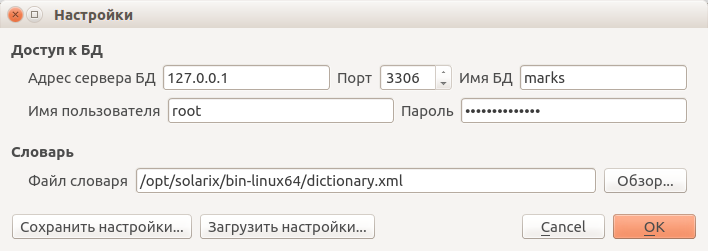
\includegraphics[scale=0.6]{pics/options.png}
\caption{Диалог настройки}
\label{fig.5}
\end{figure}

Для панели <<Доступ к БД>> указываются:

\begin{enumerate}
\item Адрес сервера БД~-- IP-адрес или доменное имя сервера базы данных;
\item Порт~-- порт доступа к БД;
\item Имя БД~-- название схемы БД с необходимыми таблицами;
\item Имя пользователя~-- имя пользователя с правами на обновление, вставку и выборку.
\item Пароль~-- пароль пользователя БД.
\end{enumerate}

Для панели <<Словарь>> поля <<Файл словаря>> указывается адрес словаря в файловой системе (стоит избегать сетевых адресов).

\subsubsection{Данные для анализа}

На странице анализа данных в качестве входных данных выступают: объект, относительно которого происходит оценка тональности информационного поля (поле <<Термин>>):

\begin{figure}[h]
\centering
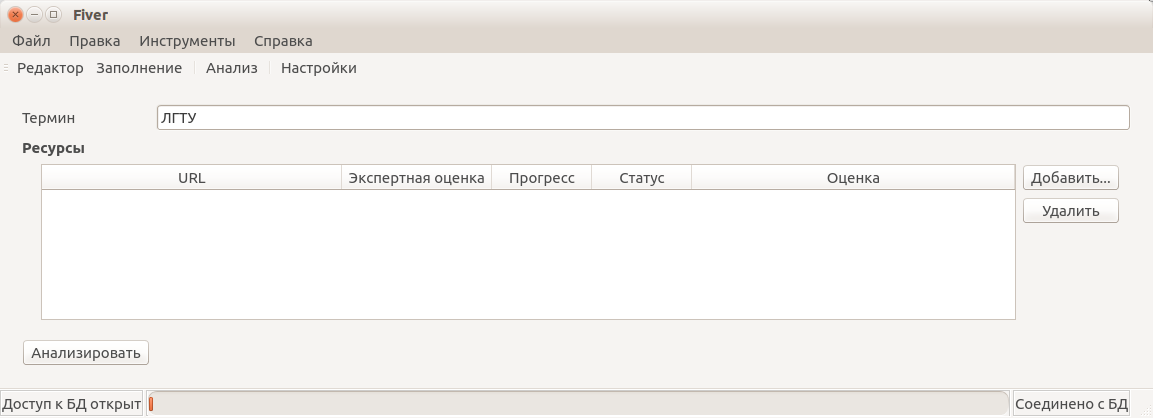
\includegraphics[scale=0.4]{pics/term.png}
\caption{Указание термина}
\label{fig.6}
\end{figure}

При нажатии на кнопку <<Добавить...>>, происходит вызов диалога для добавления документа, в котором указывается URL и экспертная оценка:

\begin{figure}[h]
\centering
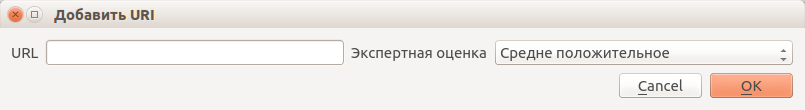
\includegraphics[scale=0.5]{pics/append_uri.png}
\caption{Диалог добавления документа}
\label{fig.7}
\end{figure}

После указания параметров документа он появится в списке анализируемых (Рис.~\ref{fig.8}).

\begin{figure}[h]
\centering
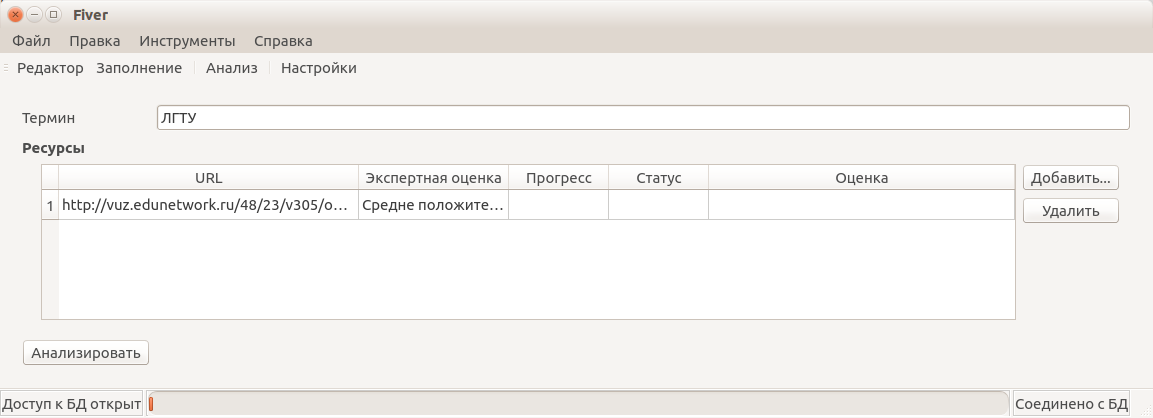
\includegraphics[scale=0.4]{pics/data_added.png}
\caption{Документ добавлен в список анализируемых}
\label{fig.8}
\end{figure}

\subsection{Выходные данные}
Для каждого документа определяется его тональность, которая отображается в графе <<Оценка>> (Рис.~\ref{fig.4}).

\begin{figure}[h]
\centering
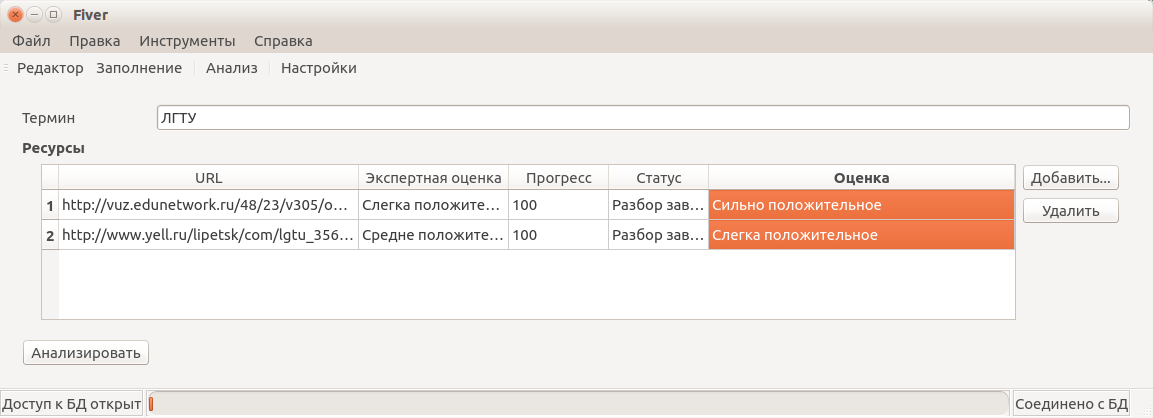
\includegraphics[scale=0.4]{pics/mark_out.png}
\caption{Выходные данные}
\label{fig.4}
\end{figure}
\section{Руководство оператора}
\subsection{Назначение программы}

Программа <<Оценка тональности документа>> предназначена для анализа эмоциональной тональности некоторого набора документов с использованием пользовательских оценок словаря.
\subsection{Условия выполнения программы}

Минимальные системные требования:

\begin{itemize}
\item Процессор x86\_x64 1 ГГц;
\item ОЗУ 2 Гб;
\item Свободное место на жестком диске~-- 10 Мб, не учитывая вес библиотек;
\item Клавиатура и мышь;
\item Монитор с разрешением не менее 640x480.
\end{itemize}

Также в ОС Linux должны быть установлены зависимости программы (устанавливаются автоматически при установке пакета; требуется соединение с Интернет).
\subsection{Выполнение программы}

Запуск программы подробно описан в соответствующих пунктах.
\subsection{Сообщения оператору}
\section{Выводы}

В данной главе содержится описание программы <<Анализ информационной тональности документа>>, разработанной для решения задач оценки информационной тональности. В главе описаны основные классы и модули программы, рассмотрены зависимости приложения, необходимые библиотеки, приведены обоснования выбора каждой из них. Означены системные требования. Приведены описания входных и выходных данных. Приведено описание процесса установки ПО, а также инструкция по работе с программой.
\newpage
\chapter{Исследование эффективности решения задачи}

\section{Формирование входных данных}

На данном этапе требуется формирование некоторого набора входных данных для анализа тональности. Следует отметить, что статьи должны обладать ярко выраженной тональностью.

\subsection{Определение ресурсов}
Сформирован список статей с ярко выраженной тональностью.

Далее следует список статей с приведенными текстами.

\subsubsection{Статья №1}

Ссылка: \url{http://vuz.edunetwork.ru/48/23/v305/opinions/}

Содержание статьи:

<<Закончила ЛГТУ в прошлом году по специальности <<вычислительная техника>>. Остались самые светлые воспоминания от учебе, не пожалела, что поступила именно сюда. Во-первых, во время учебы вуз становился все более популярным и конкурс на все специальности рос, во-вторых- качество образования- прекрасное. В-третьих, политех~-- государственный вуз, прекрасная организация досуга студентов.

Когда поступала, мне хватило баллов по ЕГЭ. Так как в среднем по математике набирают намного меньше баллов, чем по всем другим предметам, советую вам сосредоточиться именно на ней плюс физика. Баллов по 65 по этим предметам гарантирует вам поступление. Учиться не особенно трудно, так как доходчиво и понятно все объясняют на лекциях, а если возникли проблемы с пониманием~-- можно запросто подойти к любому преподавателю, благо они на кафедрах до глубокого вечера. Я этим пользовалась многократно, в итоге знания по многим предметам были даже глубже плюс налаженные контакты с преподавателями.

Практику нужно проходить на заводазх и крупных предприятиях. Здесь можно даже подзаработать.

Если вы решили учиться в ЛГТУ, то я бы посоветовал вам не выбирать гуманитарные или экономические специальности. Сам я в данный момент являюсь студентом ЛГТУ, обучаюсь на дневном платном отделении на экономическом факультете. Заканчиваю 4 курс. Выбрал специальность <<менеджмент>>, легко поступил на платное. Что касается самого вуза, то он является передовым в Липецке, да, думаю, и в области. Университет готовит разных специалистов, но преимущественно тех, кто после обучения будет работать на НЛМК. Основные корпуса находятся на окраине города, там же ректорат, общежитие, столовые, профком. Для экономистов выделили специальный корпус в центре города рядом с администрацией. Но по зданию в центре можно сказать, что оно в удовлетворительном состоянии, не более того. Что касается конкурса на место, то меня <<пугали>> тем, что на одно место приходится несколько человек. Чтобы бесплатно учиться на экономическом нужно быть льготником, другому придется платить. Количество студентов в вузе около 7500 человек. Большинство учатся на окраине, моя и еще несколько групп других специальностей в центре. Говоря об учебном процессе, хочется рассказать о преподавателях. Лично меня и моих одногруппников не устраивали бесполезные лекции, которые можно найти в интернете, а не писать 1,5 часа. Бывали случаи коллективных жалоб на преподавателей. Радует то, что преподаватели хорошо объясняют материал. За всё время обучения я не слышал чтобы кто-то давал взятку на моём факультете, преподаватели поставят минимум, даже если человек не знает ровным счетом ничего, может не с первого раза но поставит. В вузе проходят межрегиональные конкурсы, есть своя команда КВН. На нашей специальности есть 2 группы, в каждой по 12 человек. Если студент прогуливает пары, то ему за это ничего не будет, лишь бы сдал сессию, но я бы рекомендовал ходить до аттестационной недели. В вузе действует 100-бальная система оценки. Многим преподавателям и студентам она не нравится, мне в том числе. В итоге я хотел бы посоветовать, что если вы желаете учиться на экономе, то лучше выбрать другой вуз Липецка, благо их много.>>

\subsubsection{Статья №2}

Ссылка: \url{http://www.yell.ru/lipetsk/com/lgtu_3569305/}

Содержание статьи:

<<Я учусь в ЛГТУ. Не плохой институт. Преподы не берут взяток. По этому приходится всё учить. Сборные по всем видам спорта сильные. Не учёба, а просто шик.

Я учусь на 3 курсе политеха и могу сказать,что лучшее это только политех! Во-первых, самое главное для студента~-- это буфеты и столовые. Они напичканы на каждом углу и причем очень вкусная еда! Во-вторых, бесплатный интернет! В-третьих, учиться сложно, но возможно! И, в-четвертых, самодеятельность! Все услуги для студентов плюс предоставляют работу на лето. Отдых, эмоции и незабываемые впечатления!>>

\subsection{Экспертная оценка ресурсов}

Учитывая эмоциональную тональность ресурсов, для них можно выставить оценку <<Слегка положительное>> и <<Средне положительное>> соответственно для ресурсов №1 и №2. Стоит отметить, что для более точной оценки требуется привлечь несколько большее количество экспертов, но, в целом, отклонения будут находиться в пределах нормы.

\section{Анализ тональности документов}

Для проведения анализа тональности документов воспользуемся приложением Fiver. Для начала введем ссылки на статьи и предполагаемые тональности:

Запустим анализ.

\begin{figure}[h]
\centering
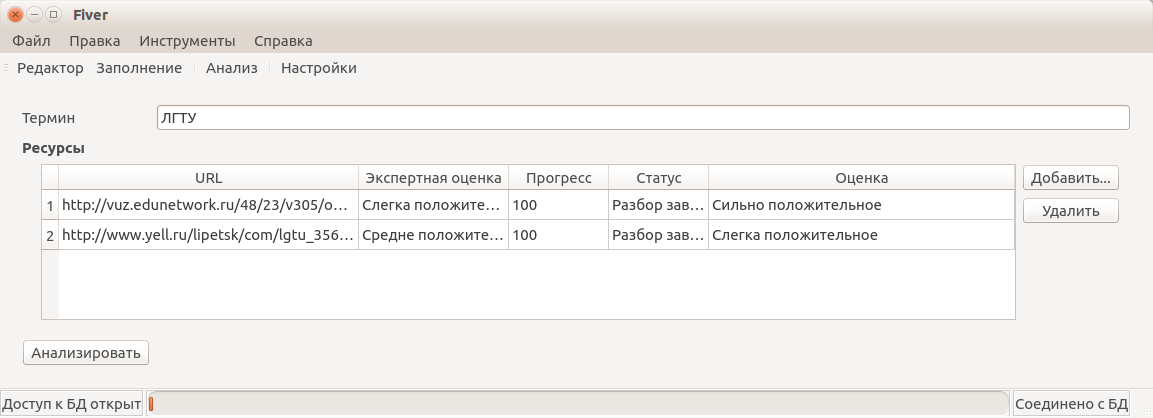
\includegraphics[scale=0.4]{pics/marking.png}
\caption{Анализ завершен}
\label{fig.1}
\end{figure}

Как видим, по завершении анализа мы получили некоторую тональность статей. Определим соответствие полученных значений и экспертных оценок.

\subsection{Определение соответствия}

Как видно, анализ статей 1 и 2 не совершенно точен, что, в первую очередь, связано как с несовершенством предложенных методов синтаксического разбора, так и с неполнотой словаря эмоциональных тональностей слов. Но, в целом, разбор показывает удовлетворительные результаты, верно оценивая общую тональность (положительно или отрицательно).

\section{Выводы}

В данной части был проанализирован некоторый набор входных данных и опытным путем эмпирически доказана корректность выбранных методов реализации приложения анализа информационной тональности документов.
\newpage
\chapter*{Заключение}
\addcontentsline{toc}{chapter}{Заключение}

Предложен основной алгоритм оценки информационной тональности некоторого документа. Разобран основной математический аппарат, применяемый для решения данной задачи.

Сформирован алгоритм, позволяющий пошагово, с помощью элементарных частей математического аппарата провести анализ эмециональной тональности некоторого документа. Рассмотрены и классифицированы методики синтаксического разбора; определены оптимальные. Проведены работы по заполнению словаря тональностей, на данном этапе покрывающего основную широко используемую мощность языка (около 4000 слов). Рассмотрен математический аппарат нечеткой логики и проведена его адаптация к основным моделям и алгоритмам математической статистики. Выбраны алгоритмы аннотирования, проведена их оценка и адаптация. Предложена модель оценки тональности текста.

Для решения поставленной задачи разработано программное обеспечение, позволяющее провести оценку эмоциональной тональности набора статей. Данное приложение также позволяет выполнять утилитарные задачи по редактированию и заполениею словаря тональностей.

С помощью программного продукта проведена оценка некоторого набора статей относительно ФГБОУ ВПО <<Липецкий государственный технический университет>>. Полученные значения совпадают с экспертными, поэтому можно сделать вывод об оптимальности решения задачи. Подводя итоги, можно сказать, что программный продукт может быть полезен широкому спектру предприятий, менеджмент которых так или иначе заитересован в оценке эмоциональной тональности документов и составлении общей картины отношения к тому или иному виду своей деятельности.

\newpage

\begin{thebibliography}{0}\addcontentsline{toc}{chapter}{Список источников}
\bibitem{blum} Нечеткая логика: алгебраические основы и приложения: монография. С. Л. Блюмин, И. А. Шуйкова, П. В. Сараев, И. В. Черпаков. Липецк: ЛЭГИ, 2002. 111 с.
\bibitem{rco} Ермаков А.Е., Киселев С.Л. Лингвистическая модель для компьютерного анализа тональности публикаций СМИ. М.: Наука, 2005. URL: \url{http://www.rco.ru/article.asp?ob_no=2340}. 10.12.2013. Загл. с экрана.
\bibitem{kondra} Кондрашова Д.С. Опыт разработки автоматического определения тональности высказываний. Вестник Московского университета. Сер.9. №3, 2010. Стр.144-151.
\bibitem{mix} Михайлов Д. В., Емельянов Г. М. Теоретические основы построения открытых вопросно-ответных систем. Семантическая эквивалентность текстов и модели их распознавания: монография. Великий Новгород: НовГУ им. Ярослава Мудрого, 2010. 286 с.
\bibitem{gubin} Губин М. В., Меркулов А. И. Эффективный алгоритм формирования контекстно-зависимых аннотаций. СПб.: ИК <<Кодекс>>, 2005. URL:\url{http://www.dialog-21.ru/Archive/2005/Gubin%20Merkulov/GubinM_MerkulovA.pdf}. 11.12.2013. Загл. с экрана.
\bibitem{fotki} API Яндекс.Фоток. URL: \url{http://api.yandex.ru/fotki/}. 08.12.2013. Загл. с экрана.
\bibitem{volk} Волкова И. А. Введение в компьютерную лингвистику. Практические аспекты создания лингвистических процессоров. М.: Издательство МГУ, 2001. 43 с.
\end{thebibliography}
\end{document}